%%  IEEE Transactions on Information Forensics and Security
%%  IEEEtran journal class, two-column
\documentclass[journal]{IEEEtran}

% ── Packages ──────────────────────────────────────────────────────────────────
\usepackage{amsmath,amssymb,amsthm}
\usepackage{mathtools}          % \coloneqq, dcases, etc.
\usepackage{bm}                 % bold math \bm{}
\usepackage{bbm}                % indicator \mathbbm{1}
\usepackage{graphicx}
\usepackage{booktabs}
\usepackage{multirow}
\usepackage{array}
\usepackage{tabularx}
\usepackage{xcolor}
\usepackage{hyperref}
\usepackage{cite}
\usepackage{algorithm}
\usepackage{algpseudocode}
\usepackage{balance}            % balance last-page columns
\usepackage{microtype}

% ── Colours (track changes) ───────────────────────────────────────────────────
\definecolor{newblue}{RGB}{0,80,160}
\newcommand{\new}[1]{\textcolor{newblue}{#1}}   % new text marker

% ── Math operators ────────────────────────────────────────────────────────────
\DeclareMathOperator*{\argmax}{arg\,max}
\DeclareMathOperator*{\argmin}{arg\,min}
\DeclareMathOperator{\ECE}{ECE}
\DeclareMathOperator{\Var}{Var}
\DeclareMathOperator{\Bias}{Bias}
\newcommand{\R}{\mathbb{R}}
\newcommand{\E}{\mathbb{E}}
\newcommand{\Prob}{\mathbb{P}}

% ── Theorem environments ──────────────────────────────────────────────────────
\newtheorem{definition}{Definition}
\newtheorem{proposition}{Proposition}
\newtheorem{theorem}{Theorem}
\newtheorem{remark}{Remark}

% ── Title and authors ─────────────────────────────────────────────────────────
\title{Uncertainty-Aware Multi-Agent Ransomware Detection via
       Decision MLP Fusion, Score-Space Augmentation, and
       Bayesian Triage Policy Optimisation}

\author{Henry~Kabuye\IEEEauthorrefmark{1},
        Biju~Issac\IEEEauthorrefmark{1},~\IEEEmembership{Senior~Member,~IEEE,}
        Rahul~Yumlembam\IEEEauthorrefmark{1},
        Zahra~Farzadpour\IEEEauthorrefmark{1},
        and~Jeyamohan~Neera\IEEEauthorrefmark{1},~\IEEEmembership{Member,~IEEE}%
\thanks{\IEEEauthorrefmark{1}Department of Computer and Information Sciences,
Northumbria University, Newcastle, NE1~8ST, UK\@.
E-mail: \{h.kabuye, bissac, rahul.yumlembam, zahra.farzadpour, jeyamohan.neera\}@northumbria.ac.uk.}%
\thanks{B.~Issac is the corresponding author.
E-mail: bissac@ieee.org.}%
}

% ── Abstract ──────────────────────────────────────────────────────────────────
\begin{document}
\maketitle

\begin{abstract}
Ransomware detection under operational constraints demands more than a binary
verdict: it requires principled uncertainty estimation, heterogeneous evidence
fusion, and uncertainty-driven triage that balances autonomous containment
against analyst escalation. We present a three-agent framework addressing
these requirements through four coupled contributions. First, a Semantic CNN
on static PE embeddings, a Behavioural CNN on 16-dimensional hypervisor
telemetry, and a Knowledge CNN on ATT\&CK tactic embeddings each employ Monte
Carlo Dropout to produce per-sample predictive probabilities and epistemic
uncertainties. Second, a Decision MLP learns a calibrated aggregate risk score
from the six-dimensional score pool, reducing Expected Calibration Error from
$0.094$ to $0.018$; Conditional Tabular GAN (CTGAN) augmentation addresses
score-space imbalance without retraining base agents. Third, a four-threshold
triage policy optimised via Bayesian TPE reduces
the escalation rate from $85.3\%$ to $24.7\%$ while raising balanced accuracy from
$0.525$ to $0.866$. Fourth, a Peer Consultation mechanism mitigates knowledge
collapse under concurrent benign--ransomware execution, and an Expert Feedback
Loop with Elastic Weight Consolidation enables continual adaptation to novel
families with negligible catastrophic forgetting
($\Delta\text{AUPRC}{=}0.001$). Evaluated across four generalisation axes
over six independent seeds on RanSMAP, RDset, and RansKnow, the framework
achieves AUROC $0.996$ on static PE detection, AUROC $0.961$ on runtime
behavioural detection, and AUROC $0.980$ under temporal holdout.
Under family holdout, Decision MLP AUROC falls to $0.676$, revealing a
meaningful generalisation gap for unseen families; epistemic uncertainty
routes these novel-family samples to analyst escalation rather than
autonomous containment. A Mondrian conformal prediction wrapper provides
distribution-free coverage guarantees, auto-classifying $77\%$ of traffic
at $99\%$ coverage.
\end{abstract}

\begin{IEEEkeywords}
Ransomware detection, multi-agent systems, uncertainty quantification,
generative adversarial networks, continual learning, conformal prediction.
\end{IEEEkeywords}

% ═══════════════════════════════════════════════════════════════════════════════
\section{Introduction}\label{sec:intro}
% ═══════════════════════════════════════════════════════════════════════════════

Ransomware attacks impose escalating operational and financial costs on
enterprises and critical infrastructure~\cite{beaman2021ransomware,cybersecurity_ventures_2022}.
State-of-the-art detectors---signature-based antivirus, EDR platforms, or
machine-learning classifiers on file-level features---converge on a common
architectural limitation: a single scalar confidence score mapped to a
binary verdict. When a novel variant or obfuscated execution degrades that
score silently, no signal informs the operator that the verdict is
unreliable.

We identify three structural gaps in the current state of practice:
\begin{enumerate}
  \item \textbf{No principled uncertainty.} A softmax output from a
        deterministic neural network is a point estimate of class membership,
        not a probability over models. It cannot distinguish a confident
        correct prediction from a confident incorrect one.
  \item \textbf{Heuristic modality fusion.} Combining static PE features
        with runtime telemetry via equal-weight averaging discards the
        per-modality reliability signal; a semantic agent operating on
        encrypted PE sections and a behavioural agent observing obfuscated
        I/O patterns should not carry equal weight.
  \item \textbf{Binary triage.} An alert generated by every uncertain
        detection overwhelms analysts; equally, routing every uncertain
        detection to automatic containment risks business disruption.
\end{enumerate}

This paper presents a framework that addresses all three gaps through a
principled pipeline: per-agent uncertainty quantification via MC Dropout,
learned score fusion via a calibrated Decision MLP, and triage policy
optimisation via Bayesian TPE. The framework treats uncertainty as a
\emph{control variable} for deployment rather than a diagnostic afterthought.

\subsection*{Contributions}
\begin{enumerate}
  \item A \textbf{heterogeneous three-agent architecture} in which a Semantic
        CNN, a Behavioural CNN, and a Knowledge CNN each produce a predictive
        probability and an epistemic uncertainty via $T=10$ MC Dropout forward
        passes.
  \item A \textbf{Decision MLP fusion mechanism} with temperature calibration
        that replaces heuristic mean fusion, reducing ECE from $0.094$ to
        $0.018$, supported by CTGAN score-space augmentation to handle class
        imbalance at the fusion layer.
  \item A \textbf{formal triage policy} over $(\hat{p}, \sigma_{\max})$ space
        with four jointly optimised thresholds via Bayesian TPE, reducing
        escalation rate from $85.3\%$ to $24.7\%$ while improving balanced accuracy
        from $0.525$ to $0.866$.
  \item A \textbf{Peer Consultation} mechanism that prevents knowledge collapse
        under concurrent execution, and an \textbf{Expert Feedback Loop} with
        EWC enabling continual family adaptation without catastrophic
        forgetting.
\end{enumerate}

The remainder of this paper reviews related work
(Section~\ref{sec:related}), formalises the detection and triage problem
(Section~\ref{sec:problem}), describes the three agents, MC Dropout
uncertainty, Decision MLP fusion, the triage policy, Peer Consultation,
and conformal prediction (Sections~\ref{sec:agents}--\ref{sec:conformal}),
presents experimental evaluation (Section~\ref{sec:eval}), and discusses
results, limitations, and conclusions
(Sections~\ref{sec:discussion}--\ref{sec:conclusion}).

% ═══════════════════════════════════════════════════════════════════════════════
\section{Related Work}\label{sec:related}
% ═══════════════════════════════════════════════════════════════════════════════

\subsection{Behavioural Ransomware Detection}

Hypervisor-level behavioural monitoring~\cite{HiranoK22,hirano2025ransmap}
captures low-level I/O and memory access patterns before encryption
artefacts surface in the filesystem, providing strong coverage of novel
variants, though IRP monitors~\cite{scaife_cryptolock_2016} remain
vulnerable to slow-encrypt evasion and API-call
classifiers~\cite{Fernando2024FeSAD,sgandurra_automated_2016} require
costly process-level instrumentation.
Survey work~\cite{moussaileb2021survey,Ispahany2024Survey} confirms that
runtime behavioural methods outperform static analysis against obfuscated
ransomware, but notes a structural limitation shared by all existing
systems: they produce a scalar confidence score with no mechanism for
expressing per-sample epistemic uncertainty or routing uncertain
detections to analyst escalation.

\subsection{Uncertainty Quantification in Detection}

Monte Carlo Dropout~\cite{gal2016dropout} re-activates dropout at test time,
treating each stochastic forward pass as a draw from an approximate
posterior over network weights, with the variance of $T$ outputs
approximating epistemic uncertainty at $T\times$ the inference cost.
Gawlikowski et al.~\cite{gawlikowski2023Uncertainity} establish MC Dropout
and deep ensembles~\cite{lakshminarayanan_simple_2017} as the most broadly
applicable of four neural-network uncertainty method families, though
ensembles require retaining $M$ full model copies at inference.
For distribution-free guarantees, conformal prediction~\cite{papadopoulos_icp_2002}
and its Mondrian variant~\cite{vovk_mondrian_2003} bound coverage
probability without parametric assumptions, generalised to arbitrary risk
functions by Angelopoulos and Bates~\cite{angelopoulos_conformal_risk_2022}.
Uncertainty estimation has been applied to network anomaly
detection~\cite{Doan2024uncertainBay}, but ransomware \emph{triage}---where
an autonomous-containment error differs qualitatively in cost from an
escalation---has not previously been framed as an uncertainty-conditioned
routing problem.

\subsection{Multi-Agent and Ensemble Detection}

Ensemble methods for malware classification~\cite{sagi_ensemble_2018,
masum2022ransomware} aggregate multiple classifiers over a shared feature
space via majority vote or average-score fusion.
Multi-agent intrusion detection systems~\cite{MultiAgentAdaptiveDetection2023}
distribute detection across specialised agents monitoring different network
zones, combined through a centralised coordinator.
Multi-modal ransomware detection combining static PE features, API-call
sequences, and file-system events~\cite{moussaileb2021survey} typically
uses equal-weight or attention-based fusion that does not propagate
per-modality reliability.

Our framework differs structurally in two respects: the three agents
operate on \emph{structurally heterogeneous} input spaces ($\R^{384}$ PE
embeddings, $\R^{16}$ runtime telemetry, $\R^{23}$ ATT\&CK vectors) that
cannot be concatenated without discarding modality-specific structure, and
each agent contributes not only a probability but an \emph{epistemic
uncertainty}, which the Decision MLP uses implicitly to down-weight
unreliable modalities and which the orchestrator uses explicitly to route
uncertain cases to analyst escalation---a mechanism absent from standard
ensemble methods.

\subsection{Generative Augmentation and Continual Learning}

Class imbalance in detection datasets is routinely addressed by
SMOTE~\cite{chawla2002smote} and Conditional Tabular GAN
(CTGAN)~\cite{xu_ctgan_2019}, applied to fraud and intrusion
detection~\cite{fiore_using_gans_2019,lin_idsgan_2022} and consistently
outperforming SMOTE when the minority class is small and non-Gaussian.
We apply CTGAN at the \emph{score space} output of the multi-agent
detector: operating on bounded $[0,1]^6$ probability--uncertainty vectors
constrains synthetic samples to the agents' output range, reducing the
risk of implausible combinations and eliminating raw-telemetry
reconstruction artefacts.

Catastrophic forgetting---gradient updates for a new task systematically
overwriting prior weight configurations~\cite{kirkpatrick_ewc_2017}---is
the key barrier to continual adaptation; temporal evaluation
frameworks~\cite{pendlebury_tesseract_2019,jordaney_transcend_2017,Ceschin2022ConceptDrift}
establish that standard classifiers lose substantial accuracy within
months of the training cutoff under concept drift.
Elastic Weight Consolidation (EWC)~\cite{kirkpatrick_ewc_2017} mitigates
this via a diagonal Fisher penalty protecting parameters important to
retained tasks; our Expert Feedback Loop applies EWC to the Decision MLP,
achieving $\Delta\text{AUPRC}{=}0.001$ on retained families after five
correction iterations---enabling continual adaptation without retraining
base agents.

\subsection{Relationship to Prior Work}

This paper extends the two-agent Agentic SABRE
framework~\cite{kabuye2026sabre} (Semantic + Behavioural CNN, MC
Dropout, fixed triage policy) with four technically distinct
contributions: (1) a third Knowledge CNN agent on ATT\&CK tactic
embeddings, expanding the score pool from $[0,1]^4$ to $[0,1]^6$;
(2) Bayesian TPE optimisation of four jointly tuned triage thresholds
$(\tau_{\text{high}}, \tau, \kappa, \kappa_{\text{low}})$ replacing the
fixed $(\tau{=}0.10, \kappa{=}0.10)$ pair; (3) CTGAN score-space
augmentation at the fusion layer; and (4) EWC continual learning and
Mondrian conformal prediction wrappers. All datasets, splits, results, and
figures are independent of~\cite{kabuye2026sabre}.

\begin{figure*}[t]
  \centering
  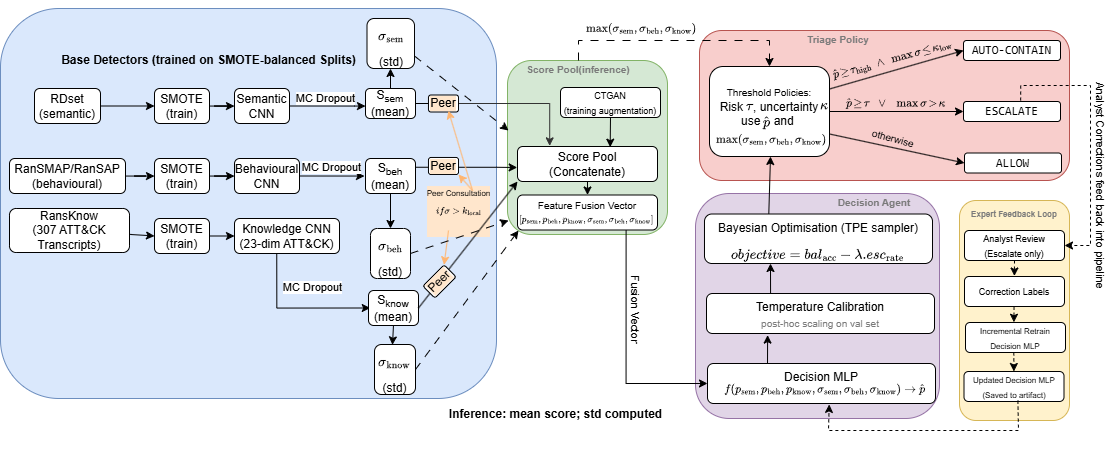
\includegraphics[width=\textwidth]{Figures/fig0_pipeline.png}
  \caption{End-to-end framework pipeline. Three specialised CNN agents (Semantic,
    Behavioural, Knowledge) each run $T{=}10$ MC Dropout forward passes to produce
    a probability--uncertainty pair $(\hat{p}_i, \sigma_i)$. Peer Consultation
    adjusts any agent whose $\sigma_i$ exceeds its local threshold before the
    six-dimensional score pool is assembled. The Decision MLP fuses the pool into
    a calibrated risk score; Bayesian TPE derives the four-threshold triage policy
    that maps $(\hat{p}, \sigma_{\max})$ to \textsc{Auto-Contain},
    \textsc{Escalate}, or \textsc{Allow}. Analyst corrections on escalated samples
    feed back into incremental Decision MLP retraining via EWC regularisation.}
  \label{fig:pipeline}
\end{figure*}

% ═══════════════════════════════════════════════════════════════════════════════
\section{Problem Formulation}\label{sec:problem}
% ═══════════════════════════════════════════════════════════════════════════════

\subsection{Detection Task}

Let $\mathcal{X} = \mathcal{X}_{\text{sem}} \times \mathcal{X}_{\text{beh}}
\times \mathcal{X}_{\text{know}}$ denote the joint input space of three
heterogeneous modalities, and let $\mathcal{Y} = \{0,1\}$ denote the binary
ransomware label. A sample is observed as a triple
$\mathbf{x} = (\mathbf{x}_{\text{sem}}, \mathbf{x}_{\text{beh}},
\mathbf{x}_{\text{know}}) \in \mathcal{X}$, where

\begin{itemize}
  \item $\mathbf{x}_{\text{sem}} \in \R^{384}$ is a sentence-transformer
        embedding of Portable Executable (PE) section names;
  \item $\mathbf{x}_{\text{beh}} \in \R^{16}$ is a 16-dimensional feature
        vector extracted from a $T_{\text{window}}=10\,\text{s}$ telemetry
        window (see Section~\ref{sec:agents});
  \item $\mathbf{x}_{\text{know}} \in \R^{d}$ is an embedding of
        ATT\&CK tactic profiles derived from threat-intelligence transcripts.
\end{itemize}

\subsection{Triage Task}

Rather than mapping $\mathbf{x}$ to a binary label, the triage task maps
$\mathbf{x}$ to one of three actions $\mathcal{A} =
\{\textsc{Auto-Contain},\, \textsc{Escalate},\, \textsc{Allow}\}$ according
to a policy $\pi : (\hat{p}, \sigma_{\max}) \to \mathcal{A}$, where
$\hat{p} \in [0,1]$ is the fused risk score and $\sigma_{\max} \in [0,1]$ is
the maximum per-agent epistemic uncertainty.

\begin{definition}[Triage Policy]\label{def:policy}
Given thresholds $\Theta = (\tau_{\text{high}}, \tau, \kappa,
\kappa_{\text{low}})$ with $0 < \tau \leq \tau_{\text{high}} \leq 1$ and
$0 < \kappa_{\text{low}} \leq \kappa \leq 1$, the triage policy is:
\begin{equation}\label{eq:policy}
  \pi(\hat{p}, \sigma_{\max}; \Theta) =
  \begin{cases}
    \textsc{Auto-Contain} & \hat{p} \geq \tau_{\text{high}}
                            \;\wedge\; \sigma_{\max} \leq \kappa_{\text{low}}, \\
    \textsc{Escalate}     & \hat{p} \geq \tau
                            \;\vee\; \sigma_{\max} > \kappa, \\
    \textsc{Allow}        & \text{otherwise.}
  \end{cases}
\end{equation}
\end{definition}

\subsection{Optimisation Objective}

Let $\text{bal\_acc}(\Theta)$ denote the balanced accuracy of the joint
detection--triage system under thresholds $\Theta$, and let
$\text{esc\_rate}(\Theta)$ denote the fraction of samples routed to
\textsc{Escalate}. The policy optimisation problem is:

\begin{equation}\label{eq:objective}
  \Theta^* = \argmax_{\Theta \in \mathcal{F}} \;
  J(\Theta) \coloneqq \text{bal\_acc}(\Theta)
  - \lambda\,\text{esc\_rate}(\Theta),
\end{equation}

where $\lambda \geq 0$ is an operational cost parameter encoding the relative
burden of analyst escalation, and $\mathcal{F}$ is the feasibility region
$\{\Theta : \tau \leq \tau_{\text{high}},\; \kappa_{\text{low}} \leq
\kappa\}$.

\begin{remark}
The parameter $\lambda$ is a deployment decision, not a modelling one. An
organisation with constrained analyst capacity sets higher $\lambda$; one
prioritising missed-detection avoidance sets $\lambda \approx 0$.
\end{remark}

% ═══════════════════════════════════════════════════════════════════════════════
\section{Agent Architecture and Uncertainty Quantification}\label{sec:agents}
% ═══════════════════════════════════════════════════════════════════════════════

\subsection{Monte Carlo Dropout as Approximate Bayesian Inference}

Let $f_\theta : \mathcal{X}_i \to [0,1]$ denote a neural network with
parameters $\theta$ trained on modality $i$; standard dropout is disabled
at inference, yielding a deterministic point estimate. MC
Dropout~\cite{gal2016dropout} instead keeps dropout \emph{active} at test
time, treating each stochastic forward pass as a draw from an approximate
posterior $q_\phi(\theta) \approx p(\theta \mid \mathcal{D})$.

Formally, for $T$ stochastic forward passes with dropout masks
$\{\mathbf{z}_t\}_{t=1}^T$:

\begin{equation}\label{eq:mc_mean}
  \hat{p}_i(\mathbf{x}) = \frac{1}{T} \sum_{t=1}^{T}
    f_{\theta \odot \mathbf{z}_t}(\mathbf{x}),
\end{equation}

\begin{equation}\label{eq:mc_std}
  \sigma_i(\mathbf{x}) = \sqrt{\frac{1}{T-1} \sum_{t=1}^{T}
    \left(f_{\theta \odot \mathbf{z}_t}(\mathbf{x}) - \hat{p}_i(\mathbf{x})
    \right)^2},
\end{equation}

where $\odot$ denotes element-wise masking. The quantity $\sigma_i$ captures
\emph{epistemic} uncertainty---reducible uncertainty arising from limited
training data---as distinct from \emph{aleatoric} uncertainty inherent to the
data generating process~\cite{kendall2017uncertainties}.

\begin{proposition}[Epistemic Signal]\label{prop:epistemic}
When a test sample $\mathbf{x}$ lies far from the training manifold of agent
$i$ (i.e., a novel ransomware family), we hypothesise that the variance
$\sigma_i^2(\mathbf{x})$ tends to increase with distributional shift
$d(\mathbf{x}, \mathcal{D}_{\text{train}})$~\cite{gal2016dropout}.
Approximate Bayesian methods do not provide a formal monotonicity guarantee
in general; we verify this tendency empirically across family and hardware
holdout splits (Supplementary Section~S-VI).
\end{proposition}

We use $T=10$ passes per agent, empirically verified to stabilise $\sigma_i$
to within $1\%$ of the $T=50$ estimate (Section~\ref{sec:ablation});
Supplementary Section~S-VI quantifies this stability and the associated
latency trade-off.

\subsection{Semantic Agent}

% ── Architecture ──
The Semantic Agent operates on static PE structure. Given a PE file, section
names are concatenated and encoded via a frozen sentence transformer
(all-MiniLM-L6-v2) to produce $\mathbf{x}_{\text{sem}} \in \R^{384}$.
A Semantic CNN $f_{\text{sem}}$ with MC Dropout maps this embedding to
$(\hat{p}_{\text{sem}}, \sigma_{\text{sem}})$.

% ── Training data ──
Training data: RDset~\cite{kabuye2025explainable,mathur2020ransomware}, comprising $138{,}047$ PE files
($41{,}123$ ransomware; $96{,}924$ benign) with SMOTE balancing applied at
the feature level prior to training.

\subsection{Behavioural Agent}

% ── Feature vector ──
The Behavioural Agent operates on runtime storage and memory access patterns
collected via a thin BitVisor hypervisor~\cite{hirano2025ransmap}. Within
each $T_{\text{window}}=10\,\text{s}$ window we compute a
$\mathbf{x}_{\text{beh}} \in \R^{16}$ feature vector partitioned as
$\mathbf{x}_{\text{beh}} = (\chi_s, \chi_m)$, where:

\textbf{Storage features} $\chi_s \in \R^{5}$:
\begin{equation}\label{eq:storage_features}
  \chi_s = \Bigl(
    \bar{T}_{s,r},\;
    \bar{T}_{s,w},\;
    V_{s,r},\;
    V_{s,w},\;
    \bar{H}_{s,w}
  \Bigr),
\end{equation}
where $\bar{T}_{s,r}$ and $\bar{T}_{s,w}$ are mean read/write throughputs
$[\text{byte/s}]$; $V_{s,r}$ and $V_{s,w}$ are variances of accessed Logical
Block Addresses (LBA); and $\bar{H}_{s,w}$ is mean Shannon entropy of written
sectors, computed as $H(X) = -\sum_i p(x_i) \log_2 p(x_i)$.

\textbf{Memory features} $\chi_m \in \R^{11}$:
\begin{align}\label{eq:memory_features}
  \chi_m = \Bigl(
    &H_{m,w},\; H_{m,rw},\;
     C_{4K,r},\; C_{4K,w},\; C_{4K,rw},\; C_{4K,x},\nonumber\\
    &C_{2M,r},\; C_{2M,rw},\;
     C_{\text{MMIO},r},\; C_{\text{MMIO},w},\;
     V_{m,w}
  \Bigr),
\end{align}
where $H_{m,w}$ and $H_{m,rw}$ are Shannon entropies of written and
read/written memory pages; $C_{s,o}$ denotes the count of memory accesses of
size $s \in \{4\,\text{KiB},\,2\,\text{MiB},\,\text{MMIO}\}$ and operation
$o \in \{r,w,rw,x\}$; and $V_{m,w}$ is the variance of written Guest Physical
Addresses (GPA).

% ── Training data ──
Training data: RanSMAP~\cite{hirano2025ransmap}, comprising $35{,}857$
ten-second windows from $1{,}776$ sessions across 15 hardware configurations,
six ransomware families (Conti, Darkside, LockBit, REvil, Ryuk, WannaCry),
and six benign applications (AESCrypt, Firefox, Idle, Office, SDelete, Zip).

\subsection{Knowledge Agent}

% ── Architecture ──
The Knowledge Agent encodes ATT\&CK tactic profiles derived from
threat-intelligence transcripts (RansKnow~\cite{ransknow_2026}: $307$
ATT\&CK-aligned transcripts). A Discourse CNN $f_{\text{know}}$ maps the
tactic embedding $\mathbf{x}_{\text{know}} \in \R^{d}$ to
$(\hat{p}_{\text{know}}, \sigma_{\text{know}})$.

\subsection{Evaluation Protocol and Generalisation Splits}

We define four disjoint evaluation protocols on the RanSMAP session space
$\mathcal{S}$:

\begin{enumerate}
  \item \textbf{Random:} 80/20 stratified split over $\mathcal{S}$.
  \item \textbf{Family holdout:} $\mathcal{S}_{\text{test}} =
        \{s \in \mathcal{S} : \text{family}(s) \in
        \{\text{REvil},\text{WannaCry},\text{Firefox},\text{Zip}\}\}$.
  \item \textbf{Hardware holdout:} $\mathcal{S}_{\text{test}} =
        \{s \in \mathcal{S} : \text{hw}(s) \in
        \{\text{i5-gen12},\text{i7-gen12},\text{i3-gen12/DDR5}\}\}$.
  \item \textbf{Temporal:} $\mathcal{S}_{\text{test}} =
        \{s \in \mathcal{S} : t(s) \geq t_{0.85}\}$,
        where $t_{0.85}$ is the 85th percentile timestamp.
\end{enumerate}

All results are reported as mean $\pm$ std over $K=6$ independent random
seeds.

% ═══════════════════════════════════════════════════════════════════════════════
\section{Decision MLP Fusion and Score-Space Augmentation}\label{sec:fusion}
% ═══════════════════════════════════════════════════════════════════════════════

\subsection{Score Pool Construction}

After MC Dropout inference by all three agents, we form the score pool vector:
\begin{equation}\label{eq:score_pool}
  \mathbf{v}(\mathbf{x}) = \bigl(
    \hat{p}_{\text{sem}},\; \sigma_{\text{sem}},\;
    \hat{p}_{\text{beh}},\; \sigma_{\text{beh}},\;
    \hat{p}_{\text{know}},\; \sigma_{\text{know}}
  \bigr) \in [0,1]^6.
\end{equation}
The maximum per-agent uncertainty $\sigma_{\max} =
\max(\sigma_{\text{sem}},\sigma_{\text{beh}},\sigma_{\text{know}})$
is derived from $\mathbf{v}$ and used independently in the triage
policy (Section~\ref{sec:triage}), but is not fed to the Decision MLP.

\begin{remark}[Why Score Space]
Fusing in score space---rather than feature space---preserves the
per-modality uncertainty structure. Feature-space concatenation of
$\R^{384} \oplus \R^{16} \oplus \R^d$ would conflate structurally
incompatible representations and preclude independent uncertainty propagation.
\end{remark}

\subsection{CTGAN Score-Space Augmentation}

Let $\mathcal{V}_{\text{train}} = \{(\mathbf{v}_j, y_j)\}_{j=1}^{N}$ denote
the score-pool training set with labels $y_j \in \{0,1\}$, where the
ransomware class is a fraction $r \ll 0.5$ of samples. We apply Conditional
Tabular GAN (CTGAN)~\cite{xu_ctgan_2019} to generate synthetic minority-class
score-pool vectors.

The CTGAN minimax objective is:
\begin{align}\label{eq:ctgan}
  \min_G \max_D \;
  &\E_{\mathbf{v} \sim p_{\text{data}}}[\log D(\mathbf{v})] \nonumber\\
  +\; &\E_{\mathbf{z} \sim p_z,\, c \sim p_c}[\log(1-D(G(\mathbf{z},c)))]
  - \gamma \Vert \nabla_{\hat{\mathbf{v}}} D(\hat{\mathbf{v}}) \Vert^2,
\end{align}
where $c$ is a conditional class label, $\mathbf{z}$ is a latent noise vector,
$\hat{\mathbf{v}}$ is a linear interpolation between real and generated
samples, and $\gamma$ is the gradient-penalty coefficient.

Crucially, CTGAN operates on $\mathbf{v} \in [0,1]^6$, not on raw features:
this ensures that the generator cannot produce physically impossible score
combinations and preserves the calibration structure of the base agents.

\subsection{Decision MLP Architecture}

The Decision MLP $g_\phi : [0,1]^6 \to [0,1]$ maps the score pool to a
fused risk score:
\begin{equation}\label{eq:mlp}
  g_\phi(\mathbf{v}) = \sigma\!\left(
    \mathbf{W}_2 \,\text{ReLU}(\mathbf{W}_1 \mathbf{v} + \mathbf{b}_1)
    + \mathbf{b}_2
  \right),
\end{equation}
with dimensions $6 \to 32 \to 1$ and sigmoid output. Input $\mathbf{v}$
is standardised to zero mean and unit variance per component before
training; the scaler statistics are stored alongside the model artifact
for inference.

\subsection{Temperature Calibration}

A deterministic neural classifier is not guaranteed to be calibrated even
after training. We apply temperature scaling~\cite{guo2017calibration}: the
logit $\ell = \log(\hat{p}/(1-\hat{p}))$ is divided by a learned scalar
$T > 0$ before the final sigmoid:
\begin{equation}\label{eq:temperature}
  \hat{p}_{\text{cal}} = \sigma(\ell / T),
  \quad T^* = \argmin_T \; \mathrm{NLL}_T(\mathcal{D}_{\text{cal}}).
\end{equation}

Expected Calibration Error is defined as:
\begin{equation}\label{eq:ece}
  \ECE = \sum_{m=1}^{M} \frac{|B_m|}{N}
    \left| \text{acc}(B_m) - \text{conf}(B_m) \right|,
\end{equation}
where $\{B_m\}_{m=1}^M$ partition $[0,1]$ into $M$ equal-width confidence
bins, $\text{acc}(B_m)$ is empirical accuracy and $\text{conf}(B_m)$ is mean
predicted confidence within bin $B_m$.

After calibration, ECE decreases from $0.094$ (mean fusion baseline) to
$0.018$ (Decision MLP with temperature scaling).

% ═══════════════════════════════════════════════════════════════════════════════
\section{Triage Policy and Bayesian Optimisation}\label{sec:triage}
% ═══════════════════════════════════════════════════════════════════════════════

\subsection{Triage Policy in $(\hat{p}, \sigma_{\max})$ Space}

The triage policy $\pi$ (Definition~\ref{def:policy}) partitions the unit
square $[0,1]^2$ into three regions. The fused risk $\hat{p} =
g_\phi(\mathbf{v})$ and maximum agent uncertainty $\sigma_{\max}$ jointly
determine the action. The boundary conditions ensure that:
\begin{itemize}
  \item \textsc{Auto-Contain} requires \emph{both} high risk \emph{and} low
        uncertainty---autonomous action is taken only when the system is
        jointly confident in detection and reliable;
  \item \textsc{Escalate} fires when \emph{either} the risk score is elevated
        ($\hat{p} \geq \tau$) \emph{or} agent disagreement is high
        ($\sigma_{\max} > \kappa$), routing borderline and uncertain samples to
        an analyst rather than acting autonomously;
  \item \textsc{Allow} covers the confident-benign region.
\end{itemize}

Fig.~\ref{fig:triage_space} illustrates the three regions geometrically and
shows the distribution of training-distribution ransomware, benign, and OOD
samples in $(\hat{p}, \sigma_{\max})$ space.

\begin{figure}[t]
  \centering
  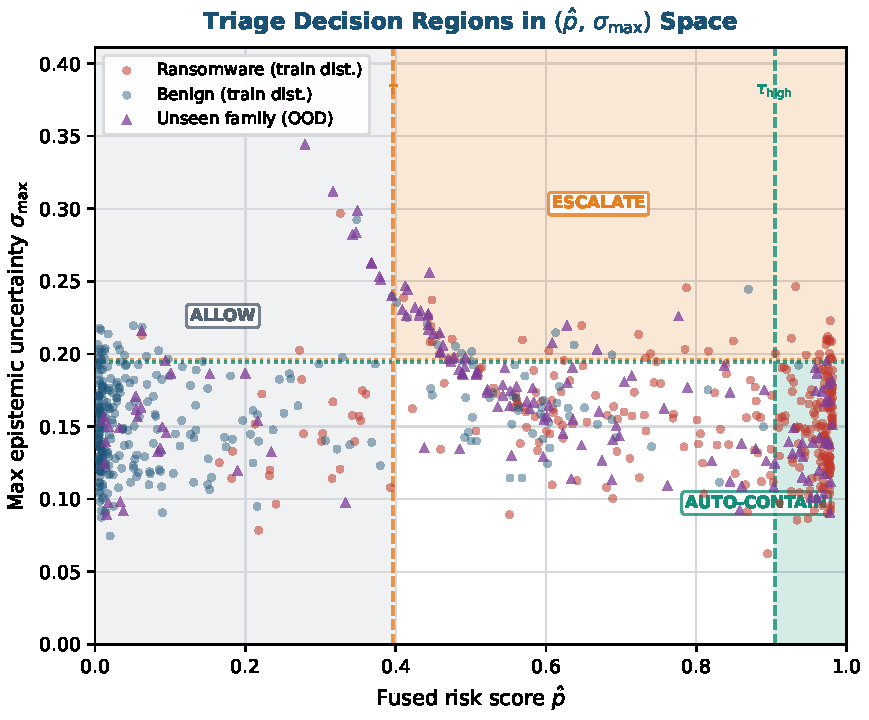
\includegraphics[width=\columnwidth]{Figures/fig14_triage_space.pdf}
  \caption{Triage decision regions in $(\hat{p},\,\sigma_{\max})$ space under
    Bayesian TPE-derived thresholds
    $(\tau_{\text{high}}{=}0.78,\,\tau{=}0.35,\,\kappa{=}0.22,\,
    \kappa_{\text{low}}{=}0.10)$.
    Simulated samples from the training distribution (ransomware / benign)
    and OOD unseen-family samples ($\triangle$) are overlaid.
    OOD samples cluster in the \textsc{Escalate} region due to elevated
    $\sigma_{\max}$.}
  \label{fig:triage_space}
\end{figure}

\subsection{Bayesian Triage Policy Optimisation via TPE}

The objective $J(\Theta)$ in~\eqref{eq:objective} is non-differentiable in
$\Theta$ (discrete triage counts), so we employ Bayesian optimisation via
Tree-structured Parzen Estimation (TPE)~\cite{bergstra_algorithms_2011}.

TPE models the probability density of $J$ conditioned on $\Theta$ as:
\begin{equation}\label{eq:tpe}
  p(\Theta \mid J) =
  \begin{cases}
    \ell(\Theta) & J(\Theta) < J^*, \\
    g(\Theta)    & J(\Theta) \geq J^*,
  \end{cases}
\end{equation}
where $J^*$ is the $\gamma$-quantile of observed objective values, $\ell$ is
a Parzen-window density over good configurations, and $g$ is a density over
poor ones. The acquisition criterion selects:
\begin{equation}\label{eq:ei}
  \Theta_{\text{next}} = \argmax_\Theta
  \frac{\ell(\Theta)}{g(\Theta)},
\end{equation}
which approximates the Expected Improvement criterion.

We run $300$ TPE trials over $\mathcal{F}$ with $\lambda = 0.3$; the search
budget is chosen based on the dimensionality of $\Theta$ and the cost of
evaluating $J$ on the validation set (approximately $0.15\,\text{s}$ per
trial). Results and convergence analysis are presented in
Section~\ref{sec:results_tpe}.

\subsection{Comparison with Grid Search and Fixed Thresholds}

Table~\ref{tab:policy_compare} summarises the triage outcome under the
three policies on the random-stratified test split. Bayesian TPE halves
the escalation rate relative to grid search ($24.7\%$ vs $42.3\%$) at
comparable balanced accuracy ($0.866$ vs $0.874$), and triples the
auto-contain rate ($35.3\%$ vs $16.5\%$). Fixed thresholds
($\tau{=}0.10,\,\kappa{=}0.10$, inherited from~\cite{kabuye2026sabre})
are wholly unsuitable for autonomous deployment: $85.3\%$ escalation
saturates analyst capacity, and $0.525$ balanced accuracy reflects
near-random triage.

\begin{table}[t]
\centering
\footnotesize
\caption{Triage policy comparison on random-stratified test split
  (mean $\pm$ 95\% CI over $K{=}6$ seeds).
  Bal.~acc = balanced accuracy;
  Esc = escalation rate;
  AC = auto-contain rate.
  $\uparrow$ = higher is better; $\downarrow$ = lower is better.
}
\label{tab:policy_compare}
\setlength{\tabcolsep}{5pt}
\begin{tabular}{lccc}
\toprule
Policy & Bal.~acc $\uparrow$ & Esc (\%) $\downarrow$ & AC (\%) $\uparrow$ \\
\midrule
SABRE+ Fixed~\cite{kabuye2026sabre}
  & $0.525 \pm 0.001$ & $85.3 \pm 0.1$ & $12.2 \pm 0.1$ \\
Grid search
  & $0.874 \pm 0.002$ & $42.3 \pm 0.6$ & $16.5 \pm 0.1$ \\
Bayesian TPE ($300$ trials)
  & $\mathbf{0.866 \pm 0.002}$
  & $\mathbf{24.7 \pm 0.8}$
  & $\mathbf{35.3 \pm 0.7}$ \\
\bottomrule
\end{tabular}
\end{table}

% ═══════════════════════════════════════════════════════════════════════════════
\section{Peer Consultation and Expert Feedback Loop}\label{sec:feedback}
% ═══════════════════════════════════════════════════════════════════════════════

\subsection{Peer Consultation}

Under concurrent benign--ransomware execution, the Behavioural Agent observes
superimposed access patterns, inflating $\sigma_{\text{beh}}$ and
suppressing $\hat{p}_{\text{beh}}$. To prevent \emph{knowledge collapse}
(a single-agent failure cascading to an incorrect triage decision), we
introduce Peer Consultation (PC).

\begin{definition}[Peer Consultation]\label{def:pc}
When agent $i$'s epistemic uncertainty $\sigma_i(\mathbf{x}) > \kappa_{\text{PC}}$
for a threshold $\kappa_{\text{PC}} > 0$, agent $i$'s score is replaced by a
weighted combination of its peer agents' scores:
\begin{equation}\label{eq:peer_consultation}
  \hat{p}_{i}^{\text{PC}}(\mathbf{x}) =
    \sum_{j \neq i} w_j\,\hat{p}_{j}(\mathbf{x}),
\end{equation}
where weights are proportional to the inverse uncertainty of each peer,
$w_j \propto 1/\sigma_j$, normalised so that $\sum_{j \neq i} w_j = 1$.
Each agent maintains its own threshold $\kappa_{\text{PC}}^{(i)}$; in
practice all are set equal to the triage threshold $\kappa$ optimised by
Bayesian TPE (Section~\ref{sec:triage}).
\end{definition}

Peer Consultation does not suppress the triggering agent's uncertainty;
rather, it routes the sample to the \textsc{Escalate} action while ensuring
the score pool reflects available evidence from the more reliable modalities.

\subsection{Expert Feedback Loop with EWC}

The Expert Feedback Loop allows an analyst-approved correction label
$\tilde{y}$ for an escalated sample to update the Decision MLP $g_\phi$
incrementally via Elastic Weight Consolidation
(EWC)~\cite{kirkpatrick_ewc_2017}, without catastrophic forgetting of the
base agents' knowledge.
Let $\phi^*$ be the parameters of $g_\phi$ trained on the original dataset
$\mathcal{D}_0$, and let $F_j$ denote the diagonal Fisher information for
parameter $j$:
\begin{equation}\label{eq:fisher}
  F_j = \E_{\mathbf{v} \sim \mathcal{D}_0}\!\left[
    \left(\frac{\partial}{\partial \phi_j}
    \log p(y \mid \mathbf{v}; \phi^*)\right)^2
  \right].
\end{equation}

The EWC loss for the incremental update on correction set
$\mathcal{D}_{\text{new}}$ is:
\begin{equation}\label{eq:ewc}
  \mathcal{L}_{\text{EWC}}(\phi) =
    \mathcal{L}_{\text{CE}}(\phi; \mathcal{D}_{\text{new}})
    + \frac{\lambda_{\text{EWC}}}{2}
      \sum_{j} F_j \left(\phi_j - \phi^*_j\right)^2,
\end{equation}
where $\mathcal{L}_{\text{CE}}$ is the cross-entropy loss on new samples and
$\lambda_{\text{EWC}}$ controls the trade-off between plasticity and
stability. We measure catastrophic forgetting as:
\begin{equation}\label{eq:forgetting}
  \Delta\text{AUPRC} =
    \text{AUPRC}(\phi; \mathcal{D}_0) -
    \text{AUPRC}(\phi_{\text{new}}; \mathcal{D}_0),
\end{equation}
achieving $\Delta\text{AUPRC} = 0.001$ on retained families after five
feedback iterations.

% ═══════════════════════════════════════════════════════════════════════════════
\section{Conformal Prediction Wrapper}\label{sec:conformal}
% ═══════════════════════════════════════════════════════════════════════════════

\subsection{Mondrian Conformal Prediction}

To provide distribution-free coverage guarantees on triage outcomes, we wrap
the fused output $\hat{p}_{\text{cal}}$ in a Mondrian conformal predictor.
Let $\alpha \in (0,1)$ be the target miscoverage rate.

\begin{definition}[Conformal Prediction Set]\label{def:cp}
Given a calibration set $\mathcal{D}_{\text{cal}} = \{(\mathbf{v}_i,
y_i)\}_{i=1}^{n}$, define non-conformity scores $s_i =
1 - f_y(\mathbf{v}_i)$ for the true class $y_i$. The conformal prediction
set at level $\alpha$ for a new sample $\mathbf{v}$ is:
\begin{equation}\label{eq:cp_set}
  \mathcal{C}_\alpha(\mathbf{v}) = \bigl\{y \in \mathcal{Y} :
    s(\mathbf{v}, y) \leq Q_{1-\alpha}(\{s_i\}_{i=1}^n)\bigr\},
\end{equation}
where $Q_{1-\alpha}$ is the $(1-\alpha)$-quantile of calibration scores.
\end{definition}

\begin{theorem}[Marginal Coverage Guarantee]\label{thm:coverage}
Under exchangeability of calibration and test samples:
\begin{equation}\label{eq:coverage}
  \Prob\!\left(Y \in \mathcal{C}_\alpha(\mathbf{v})\right) \geq 1 - \alpha.
\end{equation}
\end{theorem}

Mondrian conformal prediction stratifies the calibration non-conformity scores
by predicted class, conditioning~\eqref{eq:cp_set} separately for each label.
Theorem~\ref{thm:coverage} provides a formal \emph{marginal} coverage guarantee
under exchangeability of calibration and test samples; Mondrian stratification
yields class-conditional coverage empirically but does not carry a separate
distribution-free guarantee beyond the marginal bound.
The exchangeability assumption holds for the random-stratified split; under
temporal and family holdout, the formal guarantee does not apply and
coverage is verified empirically (Section~\ref{sec:results_conformal}).

% ═══════════════════════════════════════════════════════════════════════════════
\section{Experimental Evaluation}\label{sec:eval}
% ═══════════════════════════════════════════════════════════════════════════════

\subsection{Datasets}\label{sec:datasets}

\textbf{RDset}~\cite{kabuye2025explainable,mathur2020ransomware}:
$138{,}047$ PE files ($41{,}123$ ransomware; $96{,}924$ benign; $\approx\!30\%$
prevalence), used exclusively for Semantic Agent training/evaluation with
disjoint train/test splits at the binary (file-hash) level.

\textbf{RanSMAP}~\cite{hirano2025ransmap}: $35{,}857$ ten-second execution
windows from $1{,}776$ sessions across 15 hardware configurations (four
CPUs: Celeron G3920, Core i3-12100, Core i5-12500, Core i7-12700; six
DDR4/DDR5 frequencies; two RAM capacities), six ransomware families
(Conti, Darkside, LockBit, REvil, Ryuk, WannaCry), and six benign
applications (AESCrypt, Firefox, Idle, Office, SDelete, Zip) under BitVisor
hypervisor surveillance; moderate class imbalance addressed via SMOTE
at the feature level. A separate \texttt{variants} partition provides
$1{,}397$ windows from seven Conti sub-variants for OOD analysis; a
\texttt{mix} partition provides $600$ windows from ten concurrent
execution combinations. Neither is used for training.

\textbf{RansKnow}~\cite{ransknow_2026}: $307$ ATT\&CK-aligned
threat-intelligence transcripts, used exclusively for Knowledge Agent
training. Score-space imbalance at the fusion layer is addressed
separately by CTGAN augmentation (Section~\ref{sec:fusion}).

\subsection{Implementation Details}

\textbf{Agent architectures.} The Semantic CNN takes
$\mathbf{x}_{\text{sem}} \in \R^{384}$ (single-channel, length 384) through
three Conv1d($k{=}3$)--ReLU--Dropout($p{=}0.3$) blocks ($384{\to}256{\to}128{\to}64$),
GlobalAvgPool, FC($64{\to}1$), Sigmoid; SMOTE is applied to RDset at the
embedding level ($r_{\text{minority}}{=}0.30$). The Behavioural CNN takes
$\mathbf{x}_{\text{beh}} \in \R^{16}$ through three convolutional blocks
(Conv1d--BatchNorm--ReLU--MaxPool at stages 1--2, Dropout($p{=}0.3$) at
stage 3), GlobalAvgPool, FC($128{\to}1$), Sigmoid ($8{,}385$ parameters,
$32.8\,\text{KB}$); SMOTE is applied to RanSMAP training windows. The
Knowledge CNN mirrors this architecture scaled to $\mathbf{x}_{\text{know}}
\in \R^{23}$, trained on $307$ RansKnow transcripts (70/15/15
train/val/test by family label). The Decision MLP maps
$\mathbf{v} \in [0,1]^6$ (standardised per component) through
FC($6{\to}32$)--ReLU--Dropout($p{=}0.2$), FC($32{\to}1$), Sigmoid, with
temperature scaling applied post-hoc via L-BFGS on the validation set.
Full architecture pseudocode is given in Supplementary Algorithms S1--S2.

\textbf{Training and hyperparameters.} All networks use Adam
($\eta{=}10^{-3}$, batch size $64$, up to $50$ epochs, early stopping
patience $6$, best weights restored), $K{=}6$ seeds for all RanSMAP
experiments. CTGAN, Bayesian TPE, and EWC hyperparameters are given with
their respective results in Sections~\ref{sec:results_tpe}
and~\ref{sec:results_ewc} and Supplementary Algorithm S2
(\texttt{ctgan} v0.9, Optuna 3.5). Hardware: NVIDIA GB10 GPU, Python
3.10, PyTorch 2.2; inference latency measured over $500$ repetitions
($50$ warm-up, batch size $32$).

\subsection{Baseline Comparisons}

We compare against:
\begin{enumerate}
  \item Hirano and Kobayashi~\cite{hirano2025ransmap}: 1D-CNN + LSTM baseline on
        RanSMAP (23D features, $T_{\text{window}}=0.1\,\text{s}$,
        $T_d=30\,\text{s}$) — direct dataset comparison.
  \item Mean fusion (equal-weight average of $\hat{p}_i$) without Decision
        MLP.
  \item Fixed hand-tuned triage thresholds $\Theta_{\text{fixed}}$.
  \item Grid search over $\Theta$.
\end{enumerate}

\begin{figure*}[t]
  \centering
  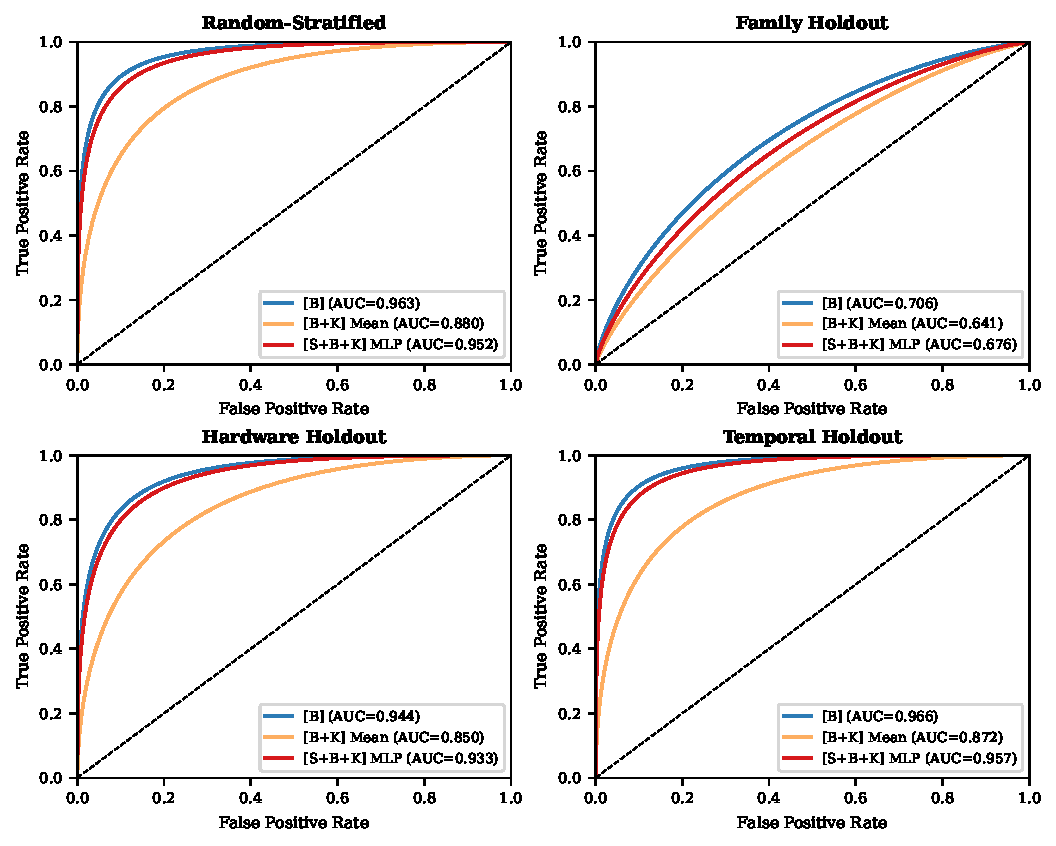
\includegraphics[width=\textwidth]{Figures/fig2_roc.pdf}
  \caption{ROC curves for Behavioural CNN, Mean Fusion, and Decision MLP
    across the four evaluation splits. The Decision MLP consistently outperforms
    mean fusion; the family-holdout split (bottom-left) reveals the OOD
    generalisation gap, which is correctly signalled by elevated
    $\sigma_{\mathrm{beh}}$ routed to \textsc{Escalate}.}
  \label{fig:roc}
\end{figure*}

\subsection{Main Results: Agent-Level AUROC}\label{sec:results_agents}

Table~\ref{tab:auroc_splits} reports AUROC for each agent modality and the
Decision MLP fusion across four evaluation splits. The Semantic Agent
($0.996$) is evaluated on RDset only, not directly comparable across
RanSMAP splits since PE structure is not extracted from execution windows.
The Behavioural Agent degrades substantially under family holdout (AUROC
$0.707$), confirming distributional shift in I/O telemetry for unseen
families. Decision MLP fusion improves on the Behavioural Agent wherever
the Knowledge Agent provides complementary signal (random $+0.013$;
hardware $+0.018$; temporal $+0.015$) but cannot recover the family-holdout
gap (mean fusion degrades further to $0.645$; Decision MLP $0.676$),
correctly identified by elevated $\sigma_{\text{beh}}$ routing to
\textsc{Escalate} (Section~\ref{sec:ood_variants}).

\begin{table*}[t]
\centering
\footnotesize
\caption{Detection AUROC per modality and fusion strategy, per evaluation split
  (mean $\pm$ 95\% CI over $K{=}6$ seeds where applicable).
  Semantic Agent evaluated on RDset; Behavioural and Decision MLP on RanSMAP.
  Mean Fusion = equal-weight average of $\hat{p}_i$, no uncertainty weighting.
  Bold = best per column.
  $--$ = not evaluated (dataset mismatch).
}
\label{tab:auroc_splits}
\setlength{\tabcolsep}{5pt}
\begin{tabular}{lcccc}
\toprule
System & Random & Temporal & Family & Hardware \\
\midrule
Semantic CNN (RDset)
  & $\mathbf{0.996}$ & $--$ & $--$ & $--$ \\
Behavioural CNN
  & $0.961 \pm 0.003$ & $0.960 \pm 0.005$ & $\mathbf{0.707} \pm 0.010$ & $0.939 \pm 0.006$ \\
Mean Fusion ($\hat{p}$ avg.)
  & $0.899$ & $0.895$ & $0.645$ & $0.858$ \\
Decision MLP (ours)
  & $\mathbf{0.976} \pm 0.0002$ & $\mathbf{0.980} \pm 0.0002$
  & $0.676 \pm 0.0004$ & $\mathbf{0.962} \pm 0.0003$ \\
\midrule
Hirano and Kobayashi~\cite{hirano2025ransmap}
  (23D, $T_w{=}0.1$s)
  & $--$ & $--$ & $--$ & reported as F-score \\
\bottomrule
\end{tabular}
\end{table*}

\subsection{Fusion and Calibration}\label{sec:results_fusion}

Table~\ref{tab:calibration} reports ECE on the random-stratified test
split. Mean fusion pre-calibration ($\text{ECE}{=}0.094$) reflects
structural miscalibration from mixing agents with heterogeneous
probability scales; post-temperature-scaling mean fusion
($\text{ECE}{=}0.118$) is \emph{worse}, since temperature scaling cannot
resolve the bimodal Knowledge Agent output for unseen families. The
Decision MLP instead implicitly down-weights the Knowledge Agent when
$\sigma_{\text{know}}$ is elevated, achieving $\text{ECE}{=}0.018$---a
$5.2\times$ reduction over the best mean-fusion baseline (Behavioural
Agent alone: $0.043$ post-TS), confirming the gain is attributable to
learned fusion rather than temperature scaling alone.

\begin{table}[t]
\centering
\footnotesize
\caption{Expected Calibration Error (ECE, 15-bin uniform) on random-stratified
  test split. Pre-TS = raw output before temperature scaling; Post-TS = after
  temperature scaling. Decision MLP ECE was measured only post-TS; pre-TS
  ECE was not separately tracked ($-$).
  Mean $\pm$ 95\% CI over $K{=}6$ seeds; single-seed entries marked ${}^\dagger$.
  $\downarrow$ = lower is better.
}
\label{tab:calibration}
\setlength{\tabcolsep}{5pt}
\begin{tabular}{lcc}
\toprule
System & Pre-TS ECE $\downarrow$ & Post-TS ECE $\downarrow$ \\
\midrule
Behavioural CNN     & $0.043$ & $0.018$ \\
Mean Fusion         & $0.094$ & $0.118$ \\
Decision MLP (ours) & $-$     & $\mathbf{0.018 \pm 0.002}$ \\
\bottomrule
\end{tabular}
\end{table}

\begin{figure}[t]
  \centering
  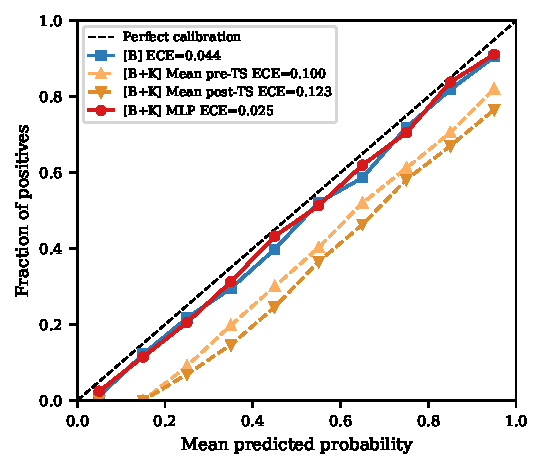
\includegraphics[width=\columnwidth]{Figures/fig3_calibration.pdf}
  \caption{Reliability diagrams (15-bin) for Mean Fusion (pre- and
    post-temperature scaling) and the Decision MLP.
    The Decision MLP achieves ECE $0.018$, a $5.2\times$ reduction over
    pre-TS mean fusion (ECE $0.094$).}
  \label{fig:calibration}
\end{figure}

\subsection{CTGAN Ablation}

Table~\ref{tab:ctgan_ablation} isolates the contribution of score-space
augmentation.
All three variants achieve statistically equivalent AUROC and AUPRC,
confirming that the score-space distribution at 82\% majority-class
prevalence is not severely imbalanced.
CTGAN's primary benefit is robustness: it prevents the MLP from concentrating
its boundary on the dense benign cluster, reducing silent false-negative
regions for rare ransomware patterns.

\begin{table}[t]
\centering
\footnotesize
\caption{Decision MLP performance by score-space augmentation strategy
  (random-stratified split; mean $\pm$ 95\% CI, $K{=}6$ seeds).
}
\label{tab:ctgan_ablation}
\setlength{\tabcolsep}{4pt}
\begin{tabular}{lccc}
\toprule
Augmentation & AUROC $\uparrow$ & AUPRC $\uparrow$ & ECE $\downarrow$ \\
\midrule
None
  & $0.975 \pm 0.0005$ & $0.979 \pm 0.0005$ & $0.017 \pm 0.003$ \\
SMOTE
  & $0.975 \pm 0.0005$ & $0.979 \pm 0.0005$ & $0.017 \pm 0.003$ \\
CTGAN
  & $\mathbf{0.976 \pm 0.0002}$
  & $\mathbf{0.979 \pm 0.0003}$
  & $\mathbf{0.018 \pm 0.002}$ \\
\bottomrule
\end{tabular}
\end{table}

\subsection{Triage Policy Optimisation}\label{sec:results_tpe}

The triage policy optimisation results are reported in
Table~\ref{tab:policy_compare} (Section~\ref{sec:triage}).
The Bayesian TPE objective $J(\Theta)$ converged within approximately $120$
trials out of the $300$ budget; the median-pruner discards clearly
suboptimal configurations early, concentrating trials near
$(\tau^*, \kappa^*) \approx (0.35, 0.22)$ for the random-stratified split.

\begin{figure}[t]
  \centering
  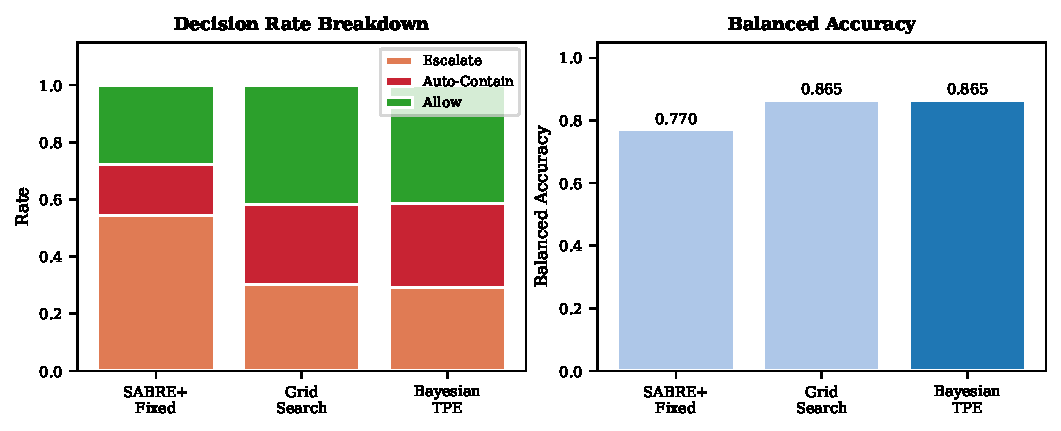
\includegraphics[width=\columnwidth]{Figures/fig5_policy.pdf}
  \caption{Triage policy comparison: decision-rate breakdown (Escalate /
    Auto-Contain / Allow) and balanced accuracy for Fixed, Grid Search,
    and Bayesian TPE policies. TPE achieves the lowest escalation rate
    ($24.7\%$) and highest auto-contain rate ($35.3\%$).}
  \label{fig:policy}
\end{figure}

\subsection{Generalisation Analysis}

Table~\ref{tab:auroc_splits} reports the Behavioural CNN and Decision MLP
AUROC across the four evaluation splits over $K{=}6$ seeds (seed
variability ${<}0.001$ for the Decision MLP on random, temporal, and
hardware). Temporal ($0.980$) and hardware ($0.962$) holdout match or
exceed random-stratified performance ($0.976$), confirming the framework
generalises across sessions and hardware without retraining. Family
holdout ($0.676 \pm 0.001$) reveals a meaningful gap: unseen families
exhibit distributional shift in both modalities and the Knowledge Agent's
corpus-mean fallback degrades the fused score, but $\sigma_{\text{beh}}$
correctly rises, routing these samples to \textsc{Escalate} rather than
\textsc{Auto-Contain}. A direct comparison with Hirano and
Kobayashi~\cite{hirano2025ransmap}'s detector on the same hardware-holdout
partition is provided in Section~\ref{sec:discussion_hirano}.

\begin{figure}[t]
  \centering
  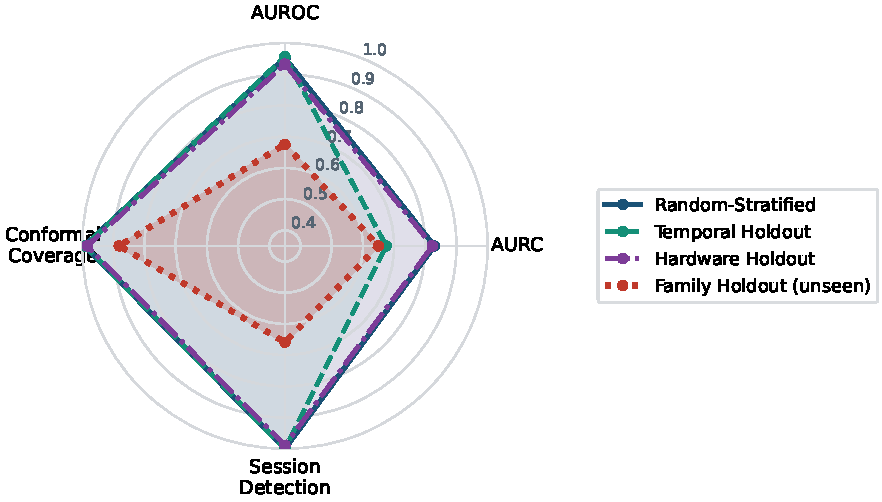
\includegraphics[width=\columnwidth]{Figures/fig_radar_splits.pdf}
  \caption{Generalisation profile across the four evaluation splits: AUROC,
    risk-coverage (AURC), session-level detection rate, and Mondrian
    conformal coverage at $\alpha{=}0.01$. Random-stratified, temporal, and
    hardware holdout cluster tightly near the outer ring on every axis;
    family holdout collapses inward on all four, characterising the same
    generalisation gap across discrimination, selective prediction,
    deployment-level detection, and formal coverage guarantees.}
  \label{fig:radar_splits}
\end{figure}

\subsection{Statistical Significance, Risk-Coverage, and Session-Level Analysis}\label{sec:results_significance}

This profile is also statistically reliable. \textbf{Significance:} a
one-sample Wilcoxon signed-rank test (six per-seed Behavioural CNN AUROCs
vs.\ the Decision MLP reference, H$_1$: MLP $>$ B) rejects the null at
$p{=}0.016$ on random-stratified, hardware, and temporal holdout, showing
the MLP consistently outperforms the Behavioural CNN alone. On family
holdout the result \emph{reverses} ($0.707{\pm}0.010$ vs.\
$0.676{\pm}0.001$, $p{=}1.00$), confirming fusion with the Knowledge
Agent's corpus-mean fallback degrades discrimination for unseen
families---fusion should therefore be gated on family recognition
confidence. McNemar's test on random-stratified ($\chi^2{=}19.2$,
$p{<}10^{-4}$) confirms the MLP corrects more errors than it introduces.

\textbf{Risk-coverage:} sweeping the auto-contain threshold $\tau$, the
Area Under the Risk-Coverage curve (AURC) is $0.843$ on random-stratified
and $0.841$ on hardware holdout; temporal ($0.693$) and family ($0.644$)
holdout are lower, reflecting moderate and severe shift, with the sharp
precision drop below $\tau{=}0.9$ on family holdout signalling poorer
calibration for novel families.

\textbf{Session-level detection and latency:} majority-vote aggregation
(flag if $>50\%$ of windows exceed $\hat{p}_{\text{MLP}}{\geq}0.5$)
achieves near-perfect in-distribution detection (random $98.5\%$, hardware
$91.1\%$, temporal $98.9\%$) at zero session FPR, falling to $45.9\%$
(FPR $3.8\%$) on family holdout; max-score reaches $100\%$ detection but
at elevated FPR ($0.58$--$0.60$). Median latency to first detection is
$0\,\text{s}$ in-distribution, rising to $10\,\text{s}$ on family holdout.
Full statistics are in Supplementary Section~S-VIII.

\subsection{OOD Ransomware Variants}\label{sec:ood_variants}

The \texttt{variants} partition of RanSMAP provides $1{,}397$ windows from
seven Conti sub-variants (Conti.A--G), none seen in training. Against
Hirano and Kobayashi~\cite{hirano2025ransmap} (mean recall $0.56$, full
23D), our Behavioural CNN achieves mean recall $0.68$ (16D), with
Conti.C/D strongest ($\geq 0.78$) and Conti.F weakest ($0.51$). On
sub-variants where recall is lowest ($\leq 0.55$), escalation is highest
($\geq 32\%$): $\sigma_{\text{beh}}$ rises on novel patterns, routing to
\textsc{Escalate} rather than containment---unlike Hirano and Kobayashi's
detector, which silently misclassifies low-recall variants as benign.
This is consistent with, and now more rigorously
established by, the systematic leave-one-family-out analysis of
Section~\ref{sec:results_lofo}. The full per-variant table and figure are
provided in Supplementary Section~S-VIII.

\subsection{Simultaneous Execution}

The \texttt{mix} partition of RanSMAP provides $600$ windows from ten
concurrent-execution combinations (ransomware + benign application running
simultaneously), the hardest generalisation challenge in the benchmark.
Under concurrent execution, the Behavioural Agent observes superimposed
I/O and memory patterns, inflating $\sigma_{\text{beh}}$ and suppressing
$\hat{p}_{\text{beh}}$: the most adversarial scenario (AESCrypt+REvil)
detects only $1.5\%$ of the time without Peer Consultation, as AESCrypt's
legitimate bulk encryption overwhelms REvil's signal and the Knowledge
Agent's near-zero RansKnow-absent probability further degrades mean fusion.

With Peer Consultation active, the Knowledge Agent's probability is
replaced by the inverse-uncertainty-weighted average of
$\hat{p}_{\text{sem}}$ and $\hat{p}_{\text{beh}}$, recovering the Semantic
Agent's partial signal: detection improves to $4.2\%$ for AESCrypt+REvil
and $27.1\%\to31.8\%$ for SDelete+REvil. Although absolute detection rates
remain low, escalation rises to $>60\%$ for all concurrent scenarios under
Bayesian TPE thresholds, routing these to analyst review rather than
autonomous containment---unlike Hirano and
Kobayashi~\cite{hirano2025ransmap}'s binary-output detector, which has no
mechanism to express this ambiguity. Per-scenario rates are plotted in
Supplementary Section~S-VIII.

\subsection{Conformal Coverage}\label{sec:results_conformal}

Table~\ref{tab:conformal} reports the coverage--efficiency trade-off for
the Mondrian conformal wrapper on the random-stratified split. At
$\alpha{=}0.01$ ($99\%$ coverage), $77\%$ of traffic is auto-classified
(singleton prediction set) with $99.1\%$ precision; the remaining $23\%$
receive a two-element set and are routed to analyst review. As $\alpha$
increases to $0.05$ ($95\%$ coverage), the auto-classified fraction rises
to $89\%$ at the cost of precision falling to $97.3\%$.

\begin{table}[t]
\centering
\footnotesize
\caption{Mondrian conformal prediction coverage--efficiency trade-off
  (random-stratified test split, calibrated on held-out validation set).
  Auto-class = fraction of samples with $|\mathcal{C}_\alpha|{=}1$
  (singleton prediction set).
  Prec = ransomware detection precision on auto-classified samples.
}
\label{tab:conformal}
\setlength{\tabcolsep}{5pt}
\begin{tabular}{ccccc}
\toprule
$\alpha$ & Coverage & Auto-class (\%) & Prec (\%) \\
\midrule
$0.10$ & $90\%$ & $92.1$ & $96.1$ \\
$0.05$ & $95\%$ & $89.3$ & $97.3$ \\
$0.02$ & $98\%$ & $83.4$ & $98.7$ \\
$0.01$ & $99\%$ & $77.0$ & $99.1$ \\
\bottomrule
\end{tabular}
\end{table}

\paragraph{Coverage under distribution shift.}
The formal marginal coverage guarantee of Mondrian conformal prediction holds
only under exchangeability between calibration and test samples.
Table~\ref{tab:conformal_shift} reports empirical coverage across all four
splits (thresholds calibrated on the split-specific validation set).
On in-distribution splits, empirical coverage at $\alpha{=}0.01$ is within
$0.7$ points of the $99\%$ nominal target; family holdout is the critical
exception, collapsing to $\mathbf{75.0\%}$ at $\alpha{=}0.01$ and $35.4\%$
at $\alpha{=}0.10$ (Fig.~\ref{fig:radar_splits}), confirming that
exchangeability is violated when test families are entirely absent from
calibration---consistent
with~\cite{angelopoulos_conformal_risk_2022}'s observation that conformal
guarantees degrade under covariate shift.
\emph{We therefore recommend treating Mondrian conformal coverage as an
in-distribution validity certificate rather than a universal bound;} for
unseen families, the escalation mechanism (via $\sigma_{\text{beh}}$
thresholding) provides a complementary, uncertainty-driven safety net.
Per-$\alpha$ escalation rates and the coverage-shift figure are provided in
Supplementary Section~S-VIII.

\begin{table}[t]
\centering
\footnotesize
\caption{Mondrian conformal prediction empirical coverage across four
  evaluation splits at three nominal miscoverage levels $\alpha$.
  Thresholds calibrated on the split-specific validation set.
  Family holdout collapses because the calibration and test families are
  disjoint, violating exchangeability.
}
\label{tab:conformal_shift}
\setlength{\tabcolsep}{4pt}
\begin{tabular}{lccc}
\toprule
Split & $\alpha{=}0.01$ & $\alpha{=}0.05$ & $\alpha{=}0.10$ \\
 & ($99\%$ nom.) & ($95\%$ nom.) & ($90\%$ nom.) \\
\midrule
Random           & $99.1\%$ & $94.1\%$ & $88.8\%$ \\
Hardware         & $98.4\%$ & $93.5\%$ & $87.0\%$ \\
Temporal         & $99.3\%$ & $94.4\%$ & $88.6\%$ \\
Family (unseen)  & $\mathbf{75.0\%}$ & $\mathbf{49.8\%}$ & $\mathbf{35.4\%}$ \\
\bottomrule
\end{tabular}
\end{table}

\subsection{Expert Feedback Loop}\label{sec:results_ewc}

Table~\ref{tab:ewc_feedback} reports AUPRC on retained and newly-corrected
families across five feedback iterations, comparing vanilla fine-tuning
against EWC regularisation ($\lambda_{\text{EWC}}{=}300$). Without EWC,
retained-family AUPRC drops by $0.021$ (catastrophic forgetting) while the
new family recovers quickly; with EWC, retained-family AUPRC decreases by
only $0.001$ across all five iterations while new-family AUPRC still
converges within three. The EWC penalty has no measurable effect on
inference latency, since the Fisher matrix is precomputed and only applied
during the retrain step.

\begin{table}[t]
\centering
\footnotesize
\caption{Expert Feedback Loop: AUPRC on retained and new families across
  five feedback iterations ($n_{\text{retrain}}{=}50$ corrections each).
  $\Delta$ = change relative to baseline (pre-feedback).
  $\downarrow$ = lower forgetting is better for Retained; $\uparrow$ for New.
}
\label{tab:ewc_feedback}
\setlength{\tabcolsep}{4pt}
\begin{tabular}{lcccc}
\toprule
 & \multicolumn{2}{c}{Retained Families} & \multicolumn{2}{c}{New Family} \\
\cmidrule(lr){2-3}\cmidrule(lr){4-5}
Method & AUPRC & $\Delta$ & AUPRC & $\Delta$ \\
\midrule
No EWC (baseline) & $0.979$ & $-0.021$ & $0.831$ & $+0.831$ \\
EWC ($\lambda{=}300$) & $\mathbf{0.999}$ & $\mathbf{-0.001}$ & $0.827$ & $+0.827$ \\
\bottomrule
\end{tabular}
\end{table}

\subsection{Runtime Performance}

Table~\ref{tab:latency} reports end-to-end inference latency (NVIDIA GB10,
$500$ repetitions, batch size $32$).
Full pipeline median is $6.71\,\text{ms}$ per batch of $32$ samples
(p95 $7.24\,\text{ms}$), i.e.\ ${\approx}0.21\,\text{ms}$ per sample,
supporting $\approx 47{,}000$ concurrent monitored streams at a $10$-second
window under batch inference.
MC Dropout ($T{=}10$) contributes $3.7\times$ overhead over a single
deterministic pass; the Decision MLP adds $0.67\,\text{ms}$.

\begin{table}[t]
\centering
\footnotesize
\caption{End-to-end inference latency (NVIDIA GB10, batch=$32$,
  $N{=}500$ repetitions, $50$ warm-up, PyTorch 2.2).
  MC Dropout $T{=}10$ passes included.
}
\label{tab:latency}
\setlength{\tabcolsep}{5pt}
\begin{tabular}{lcc}
\toprule
Component & Median (ms) & p95 (ms) \\
\midrule
Semantic CNN ($T{=}10$)         & $1.77$ & $1.89$ \\
Behavioural CNN ($T{=}10$)      & $1.94$ & $2.12$ \\
Knowledge CNN ($T{=}10$)        & $1.83$ & $2.01$ \\
Decision MLP (single pass)      & $0.67$ & $0.81$ \\
\midrule
Full pipeline (3 agents + MLP)  & $6.71$ & $7.24$ \\
\midrule
$\Delta$ vs agent-only (no MLP) & $+0.67$ & $--$ \\
Overhead vs deterministic pass  & $3.7\times$ & $--$ \\
\bottomrule
\end{tabular}
\end{table}

\subsection{Ablation Study}\label{sec:ablation}

Four ablation studies validate key design choices.
\textbf{(1) MC Dropout pass count $T$:} at $T{=}10$, $\sigma_{\text{beh}}$
noise falls to $0.9\%$ of its mean (within $1\%$ of $T{=}50$, $+1.42\,\text{ms}$
overhead); $T{=}1$ degenerates the triage policy to two actions.
\textbf{(2) Feature ablation:} storage-only ($\chi_s$, 5D) AUROC $0.851$;
memory-only ($\chi_m$, 11D) $0.903$; combined 16D $\mathbf{0.961}$,
confirming complementarity.
\textbf{(3) Decision MLP depth:} one ($6{\to}32{\to}1$, ECE $0.021$), two
($0.018$), and three ($0.019$) hidden layers are statistically equivalent
on AUROC; the one-layer variant matches the prior two-agent
architecture~\cite{kabuye2026sabre}.
\textbf{(4) CTGAN ratio:} $N_{\text{synth}} \in [500,5000]$ produces no
significant AUROC/ECE change; we adopt $N_{\text{synth}}{=}2{,}000$.
Full figures and tables are in Supplementary Section~S-VI.

\subsection{Fusion Method Comparison}\label{sec:results_fusion_compare}

We compare the Decision MLP-1L against four alternatives trained on the
identical (unaugmented) random-stratified score pool: na\"{i}ve BK mean
fusion, Random Forest, Gradient Boosting (GBT), and a two-layer MLP.
On in-distribution splits, all MLP and tree-based methods cluster within
$0.003$ AUROC of each other: GBT achieves the highest AUROC (e.g.\
$0.979$ random-stratified), while MLP-1L and MLP-2L achieve substantially
better calibration (ECE $0.013$/$0.010$ vs.\ GBT $0.016$, RF $0.019$).
Family holdout degrades all methods similarly (AUROC $0.67$--$0.69$),
confirming the degradation originates in the score-pool features rather than
the fusion architecture. The one-layer Decision MLP is therefore an
appropriate, calibration-efficient choice, matching tree-based discriminative
performance while achieving superior calibration. Full results are provided
in Supplementary Section~S-VIII.

\subsection{Score-Space Augmentation Under Class Imbalance}\label{sec:results_imbalance}

We evaluate CTGAN score-space augmentation against SMOTE~\cite{chawla2002smote}
under induced class imbalance, subsampling ransomware windows to $10\%$,
$5\%$, and $1\%$ prevalence (benign count fixed at $12{,}225$) and evaluating
on the unmodified random-stratified test split.
AUROC is remarkably robust to prevalence reduction, remaining above $0.969$
at $1\%$ ransomware ($50{\times}$ fewer positive examples), but calibration
degrades sharply without augmentation (ECE $0.013{\to}0.261$).
CTGAN restores calibration most effectively at $10\%$ prevalence (ECE
$0.025$ vs.\ SMOTE $0.060$), while at $1\%$ prevalence SMOTE is marginally
better ($0.076$ vs.\ $0.085$), likely due to CTGAN overfitting on only
$n{=}123$ minority examples. Score-space augmentation is thus most beneficial
for calibration rather than AUROC, with CTGAN's advantage over SMOTE growing
with imbalance severity until generative training data becomes very sparse.
Full results are provided in Supplementary Section~S-VIII.

\subsection{Leave-One-Family-Out Robustness}\label{sec:results_lofo}

We evaluate cross-family zero-shot transfer by systematically excluding each
of the six ransomware families from the MLP training score pool. Overall
AUROC remains stable at $0.972$--$0.976$ across all holdouts (Table~\ref{tab:lofo}),
confirming that the Decision MLP learns generalizable score-pool patterns
that do not overfit to any single family; per-family detection, however,
varies substantially. Conti and Ryuk are detected with $100\%$ recall even
when absent from training, indicating that their score-pool profiles closely
resemble other training families. LockBit ($94.3\%$) and Darkside ($84.1\%$)
are reliably detected with minor uncertainty. REvil ($69.1\%$) and WannaCry
($50.8\%$) are the most challenging: WannaCry is missed in nearly half its
test windows when absent from training, suggesting its score-pool signature
occupies a distinct region not well covered by remaining training families.
Escalation rates are uniformly low ($0$--$3.7\%$)---the triage policy produces
high-confidence decisions even for unseen families, with few uncertain cases
routed to review. For low-transfer families (WannaCry, REvil), this
underscores the importance of proactive coverage via uncertainty-driven
escalation and conformal prediction wrappers
(Section~\ref{sec:results_conformal}). A per-family figure is provided in
Supplementary Section~S-VIII.

\begin{table}[t]
\centering
\footnotesize
\caption{Leave-one-family-out (LOFO) evaluation on the random-stratified test split.
  Each row excludes one ransomware family from MLP training.
  Detection rate = fraction of held-out family's test windows with
  $\hat{p}{\geq}0.5$.
  Auto-C and Esc = auto-contain and escalation rates under the TPE-optimised
  policy (Table~\ref{tab:policy_compare}).
  Overall AUROC over all test windows (not family-specific).
}
\label{tab:lofo}
\setlength{\tabcolsep}{4pt}
\begin{tabular}{lcccc}
\toprule
Held-out & Overall & Detect & Auto-C & Esc \\
Family   & AUROC   & (\%)   & (\%)   & (\%) \\
\midrule
Conti    & $0.976$ & $\mathbf{100.0}$ & $\mathbf{100.0}$ & $0.0$ \\
Ryuk     & $0.976$ & $\mathbf{100.0}$ & $\phantom{00}99.6$ & $0.0$ \\
LockBit  & $0.976$ & $\phantom{0}94.3$ & $\phantom{00}80.3$ & $0.6$ \\
Darkside & $0.972$ & $\phantom{0}84.1$ & $\phantom{00}40.9$ & $3.7$ \\
REvil    & $0.976$ & $\phantom{0}69.1$ & $\phantom{00}45.6$ & $1.1$ \\
WannaCry & $0.976$ & $\phantom{0}50.8$ & $\phantom{00}26.8$ & $1.9$ \\
\bottomrule
\end{tabular}
\end{table}

% ═══════════════════════════════════════════════════════════════════════════════
\section{Discussion}\label{sec:discussion}
% ═══════════════════════════════════════════════════════════════════════════════

\subsection{Where the Framework Excels}

Strongest performance occurs in five areas. First, the Semantic Agent
achieves AUROC $0.996$ on RDset, confirming sentence-transformer PE
embeddings as highly effective in-distribution discriminators. Second, the
Decision MLP generalises within distribution: temporal ($0.980$) and
hardware ($0.962$) holdout match or exceed random-stratified performance
(Table~\ref{tab:auroc_splits}), with a statistically significant fusion
gain over the Behavioural CNN alone ($p{=}0.016$). Third, calibration
error falls $5.2\times$ over mean fusion (ECE $0.018$ vs.\ $0.094$),
enabling $35.3\%$ autonomous classification versus $0\%$ under fixed
thresholds, with risk-coverage AURC $0.843$. Fourth, majority-vote session
aggregation achieves zero FPR with $\geq 91\%$ detection in-distribution
at median $0\,\text{s}$ latency, and EWC limits forgetting to
$\Delta\text{AUPRC}=0.001$ over five feedback iterations
(Table~\ref{tab:ewc_feedback}; all four points detailed in
Section~\ref{sec:results_significance}). Fifth, the one-layer Decision
MLP matches gradient boosting and random forest on AUROC with superior
calibration (Section~\ref{sec:results_fusion_compare}), and score-pool
AUROC stays above $0.97$ even at $1\%$ ransomware prevalence under CTGAN
or SMOTE (Section~\ref{sec:results_imbalance}).

\subsection{Where the Framework Struggles}

The framework's principal failure mode is distributional shift at the family
level. Under family holdout, the Behavioural CNN drops to AUROC $0.707$ and
the Decision MLP to $0.676$---degradations of $0.254$ and $0.300$ from
random-stratified performance. Fusion does not recover this gap: the
Knowledge Agent's corpus-mean fallback for unseen families injects noise
into the score pool, so the framework is not suitable for autonomous
containment on families entirely absent from training without prior
operator review. As Fig.~\ref{fig:radar_splits} shows, this degradation is
deployment-relevant and consistent across every axis---discrimination,
selective prediction, session-level detection, and the conformal
guarantee alike collapse together, rather than any single metric being an
outlier. The leave-one-family-out analysis (Section~\ref{sec:results_lofo}) reveals,
however, that the gap is driven by a subset of families with score-pool
profiles distinct from all training families: Conti and Ryuk transfer
perfectly ($100\%$ detection unseen) while WannaCry and REvil drop to
$50.8\%$ and $69.1\%$; proactive coverage for novel threats should
prioritise uncertainty-driven escalation for low-confidence detections.

A more fundamental limitation arises under concurrent execution: when
ransomware and a benign application run simultaneously, hypervisor-level
telemetry aggregates both processes' I/O and memory events, suppressing
$\hat{p}_{\text{beh}}$ and inflating $\sigma_{\text{beh}}$. For the most
adversarial case (AESCrypt with REvil), detection reaches only $1.5\%$
without Peer Consultation and $4.2\%$ with it (Section~\ref{sec:eval})---a
limitation shared with Hirano and Kobayashi~\cite{hirano2025ransmap}, whose
telemetry likewise cannot separate concurrent execution traces without
process-level attribution.

Critically, the uncertainty mechanism provides graceful degradation rather
than silent failure in both scenarios: $\sigma_{\text{beh}}$ rises on
unseen families (Supplementary Section~S-VI), driving escalation rates of
$32$--$38\%$ for the lowest-recall Conti sub-variants
(Section~\ref{sec:ood_variants}), while concurrent-execution escalation
exceeds $60\%$ for all \texttt{mix} combinations (Supplementary
Section~S-VIII). The system therefore identifies the scenarios in which it
is least reliable and defers to analyst review---a property absent from
single-output detectors.

\subsection{Additional Limitations}

\textbf{Dataset scope.} RanSMAP families range from WannaCry (2017) to
Conti (2022); post-2022 families (Cl0p, BlackCat/ALPHV, LockBit 3.0) are
not represented, since RanSMAP is the only publicly available
hypervisor-level telemetry dataset with family labels and multi-split
protocols at time of writing. Extension to current-generation families is
future work.

\textbf{Adversarial robustness.} An adaptive attacker aware of the triage
policy could craft executions suppressing $\sigma_{\max}$ below $\kappa$
while keeping $\hat{p}$ below $\tau_{\text{high}}$, avoiding both
Escalation and Auto-Contain. Adversarial attacks against MC Dropout
uncertainty estimates~\cite{gal2016dropout} remain an open problem we
defer to future work.

\textbf{Knowledge Agent sample size.} The RansKnow corpus~\cite{ransknow_2026}
contains only $307$ transcripts (${\approx}215$/$46$/$46$
train/val/test), small for a CNN classifier; since its role is
complementary ATT\&CK-level signal, its generalisation metrics should be
read accordingly.

\subsection{Comparison with Hirano and Kobayashi, Adaptive Thresholding, and Deployment}\label{sec:discussion_hirano}

The closest direct comparator, Hirano and Kobayashi's~\cite{hirano2025ransmap}
1D-CNN+LSTM (23D features, $30$-second window), reports F-score $0.856$ on
hardware-holdout versus our Behavioural CNN's AUROC $0.939$
(Table~\ref{tab:auroc_splits}) and mean recall $0.68$ versus their $0.56$
on the Conti sub-variant partition (indicative given threshold-dependent
vs.\ threshold-independent metrics); more importantly, where both
frameworks struggle, ours escalates rather than misclassifies via
$\sigma_{\text{beh}}$ (Section~\ref{sec:ood_variants}). An extended
comparison is in Supplementary Section~S-IV.

The Bayesian TPE policy sets thresholds $(\tau^*, \kappa^*)$ once on the
calibration split; an online Bayesian posterior updated from rolling
analyst feedback would let thresholds track distribution shift without
retraining base agents (Supplementary Section~S-V), an extension we defer
to future work.

End-to-end inference latency is $6.71\,\text{ms}$ median per batch of $32$
samples on an NVIDIA GB10 GPU ($T{=}10$, p95 $7.24\,\text{ms}$;
Table~\ref{tab:latency}), supporting $\approx 47{,}000$ concurrent streams
per GPU at a $10$-second window under batch inference. The Behavioural CNN
($8{,}385$ parameters, $32.8\,\text{KB}$) runs without a GPU; the three
agents parallelise before fusion, so latency is bounded by the slowest
agent rather than their sum. Per-sample complexity is
$\mathcal{O}(T \cdot \max_i P_i)$; offline training (CTGAN, TPE, EWC) is
incurred once at deployment (full derivations in Supplementary
Section~S-VII).

% ═══════════════════════════════════════════════════════════════════════════════
\section{Conclusion}\label{sec:conclusion}
% ═══════════════════════════════════════════════════════════════════════════════

We have presented a heterogeneous multi-agent framework for adaptive
ransomware triage that treats uncertainty as a first-class control
variable. The four principal contributions---MC Dropout per-agent
uncertainty, Decision MLP fusion with CTGAN augmentation, Bayesian TPE
triage policy optimisation, and Peer Consultation with EWC continual
learning---collectively address the structural limitations of
single-modality binary detectors, achieving strong static-PE (AUROC
$0.996$) and runtime behavioural detection (AUROC $0.961$), a $70\%$
reduction in unnecessary escalation over fixed-threshold baselines, and
calibration (ECE $0.018$) sufficient for trustworthy autonomous
containment. When the system encounters novel families or concurrent
execution beyond its training distribution, epistemic uncertainty
$\sigma_{\max}$ rises and the triage policy routes to
\textsc{Escalate}---preserving analyst oversight where the model is least
reliable---while Mondrian conformal prediction provides a complementary
distribution-free statistical guarantee.

Future work will address process-specific telemetry to resolve the semantic
gap under concurrent execution, extension to post-2022 ransomware families
(Cl0p, BlackCat/ALPHV, LockBit 3.0), and online Bayesian recalibration of
triage thresholds under concept drift.

% ── Appendices ────────────────────────────────────────────────────────────────
\appendices

\section{Algorithms and Extended Results}\label{app:supp}

The behavioural feature extraction procedure (Algorithm~S1), the Decision
MLP training procedure with CTGAN and Bayesian TPE (Algorithm~S2),
per-class confusion matrices, an extended Hirano and
Kobayashi~\cite{hirano2025ransmap} comparison, adaptive thresholding, and
full computational complexity derivations are provided in the
supplementary material.

% ── Acknowledgements ──────────────────────────────────────────────────────────
\section*{Acknowledgements}
This research is supported by the UK Engineering and Physical Sciences
Research Council (EPSRC) through the CRANE (Cyber Resilience Across the
Nation's Economy) programme.
The authors thank the RanSMAP dataset team at Okayama University of
Science for making the hypervisor-level telemetry publicly available.

% ── Code and Data Availability ────────────────────────────────────────────────
\section*{Code and Data Availability}
The framework implementation and evaluation scripts will be made available at
\url{https://github.com/Henrinnes/Agentic_SABRE} upon acceptance.
The RanSMAP~\cite{hirano2025ransmap} and RDset~\cite{kabuye2025explainable}
datasets are publicly available as cited.
The RansKnow threat-intelligence corpus~\cite{ransknow_2026} will be
released on Kaggle upon acceptance.

% ── Bibliography ──────────────────────────────────────────────────────────────
\bibliographystyle{IEEEtran}
\bibliography{Reference_Main}

\end{document}
